\documentclass{article}
\usepackage[T2A]{fontenc}
\usepackage{float}
\usepackage{geometry}
\geometry{
	a4paper,
	top=25mm, 
	right=15mm, 
	bottom=25mm, 
	left=30mm
}


\usepackage{graphicx} % Required for inserting images
\usepackage{amsmath}
\usepackage[english,russian]{babel}

\title{Работа 1.1.1\\ 
	Определение систематических и случайных погрешностей при измерении удельного сопротивления нихромовой проволоки}


\begin{document}
	
	\maketitle
	
	\section{Аннотация}
	В работе измеряется удельное сопротивление нихромовой проволоки двумя способами: 1) путем анализа графика ВАХ проволоки, 2) путем вычисления по известной формуле \(R = \rho \frac{l}{S}\), где \( R\) измерено  посредством моста Уильсона (моста постоянного тока).\\\\
	\emph{Цель работы:} измерить удельное соединение нихромовой проволоки и вычислить систематические и случайные погрешности при использовании измерительных прибров. \\\\
	\emph{Оборудование:} линейка, штангенциркуль, микрометр, нихромовая проволока, амперметр, стрелочный вольтметр, источник ЭДС, мост Уильсона (мост постоянного тока), реостат, ключ, провода.
	
	\section{Теоретические сведения}
	
	Удельное сопротивление цилиндрической проволоки определяется по формуле:
	$ \rho = \frac{R}{l}S $, а учитывая что $ S = {\pi}{\frac{d^2}{4}} $,
	
	$$ \rho = \frac{R}{l}{\frac{{\pi}d^2}{4}} $$
	Где $ R $ - сопротивление отрезка проволоки, $ l $ - его длина, $ d $ - диаметр.\\\\
	По закону Ома для участка цепи: 
	$$ R = \frac{U}{I} $$
	$ U $ - напряжение на участке цепи, $ I $ - сила тока, $ R $ - сопротивление.\\
	
	Таким образом, для определения сопротивления проволоки достаточно измерить силу тока и напряжение на нем. Это возможно с помощью схемы рис.1.\\
	\begin{figure}
		\centering
		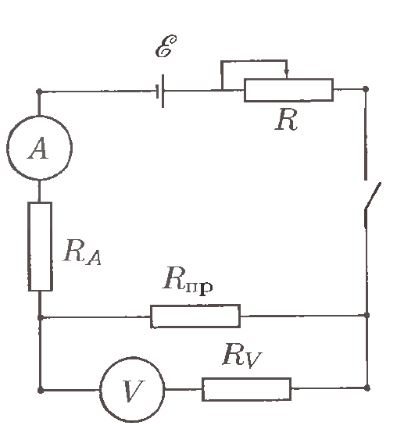
\includegraphics[width = 0.5\linewidth]{1.png}
		\caption{Используемая схема}
		\label{fig:enter-label}
	\end{figure}
	
	Вольтметр верно измеряет падение напряжения на проволоке, а амперметр измеряет сумму токов через проволоку и вольтметр. Поэтому можно записать систему:\\
	\begin{equation}
		\begin{cases}
			$$ I_{A} = I + I_{V} $$\\
			$$IR = U_{V} $$\\
			$$I_{V}R_{V} = U_{V} $$
		\end{cases} 
	\end{equation}
	$U_{V}$ - показания вольтметра, $I_{A}$ - показания амперметра\\\\
	Выразив токи $I$ и $I_{V}$ и подставив их в первое уравнение получим\\
	\begin{equation}
		\label{R_fake}
		R_{\text{1}} = \frac{U_{V}}{I_{A}}= R\frac{R_{V}}{R+R_{V}}
	\end{equation}
	Здесь $R_{1}$ не является истинным сопротивлением проволоки, выразим истинное сопротивление $R$ из (\ref{R_fake}):
	
	$$R = \frac{R_{1}}{1 - \frac{R_{1}}{R_{V}}}$$
	В силу величины $R_{V}$ по сравнению с $R_{1}$:
	
	\begin{equation}
		R \approx R_{1}(1 + \frac{R_{1}}{R_{V}})
	\end{equation}
	
	
	
	\section{Оборудование и экспериментальные погрешности}
	
	\emph{Линейка}: $\Delta_{\text{лин}} = \pm 0.5$ мм (половина цены деления)\\
	\emph{Штангенциркуль}: $\Delta_{\text{шт}} = \pm 0.05$ мм (половина цены деления)\\
	\emph{Микрометр}: $\Delta_{\text{мкм}} = \pm 0.01$ мм (маркировка производителя)\\
	\emph{Амперметр}: $\Delta_{\text{А}} = \pm (0.002 * X + 2k)$, где X - измеряемая величина, k - единица младшего разряда (k = 0.01 мА) (согласно паспорту прибора)\\
	\emph{Вольтметр}: $\Delta_{\text{V паспорт}} = \pm (0.005 * X)$, где X - измеряемая величина (согласно классу точности)\\
	Т.к. положение стрелки вольтметра определялось на глаз, к погрешности вольтметра можно прибавить половину цены деления :\\
	$$\Delta_{\text{V}} = \pm (0.005 * X + 0.5 * c),$$ где c - цена деления
	
	\section{Измерения и обработка данных}
	
	\subsection{Измерение длины проволоки $l$}
	Значения $l$ измерялись с помощью линейки.\\
	$\Delta_{\text{l}} = 2\Delta_{\text{лин}} = \pm 1\text{ мм}$ (т.к. оба конца проволоки не были зафиксированы)
	
	\subsection{Измерение диаметра проволоки $d$}
	Проволока неоднородна, поэтому ее диаметр различен в разных местах. Мы можем измерить его в нескольких местах и усреднить полученные значения.\\\\
	Измерения с помощью штангенциркуля показали одинаковый диаметр проволоки для $N = 12$ измерений, $d_{\text{шт}} = 0.4 \text{мм}$.\\
	
	\begin{table}[H]
		\centering
		\begin{tabular}{|c|c|c|c|c|c|c|c|c|c|c|c|c|}
			\hline
			№ & 1 & 2 & 3 & 4 & 5 & 6 & 7 & 8 & 9 & 10 & 11 & 12 \\ \hline
			$d_{\text{шт}}$, мм & 0.4 & 0.4 & 0.4 & 0.4 & 0.4 & 0.4 & 0.4 & 0.4 & 0.4 & 0.4 & 0.4 & 0.4 \\ \hline
		\end{tabular}
		\caption{Результат измерения $d$ штангенциркулем}
	\end{table}
	Для измерения диаметра был также использован микрометр, который выявил отличия в диаметре проволоки в разных ее местах (см. Табл. 1).
	
	\begin{table}[H]
		
		\centering
		\begin{tabular}{|c|c|c|c|c|c|c|c|c|c|c|c|c|}
			\hline
			№ & 1 & 2 & 3 & 4 & 5 & 6 & 7 & 8 & 9 & 10 & 11 & 12 \\ \hline
			$d_{\text{мкм}}$, мкм & 380 & 380 & 360 & 390 & 360 & 370 & 350 & 340 & 360 & 380 & 370 & 370 \\ \hline
		\end{tabular}
		\caption{Результат измерения $d$ микрометром}
	\end{table}
	Средний диаметр $$\overline{d} = \frac{\Sigma d_{i}}{N} = 367.5 \text{ мкм}$$\\
	Среднее квадратичное отклонение $$\sigma_{d} = \sqrt{\frac{1}{N}\sum_{i = 1}^{N} \Delta d^{2}_{i}} = 13.62 \text{ мкм}$$\\
	Погрешность среднего $$\sigma_{\overline{d}} = \frac{\sigma_{d}}{\sqrt{N}} = 3.93 \text{ мкм}$$
	Общая погрешность $$\sigma_{d} = \sqrt{\sigma_{\overline{d}}^{2} + \Delta_{\text{мкм}}^{2}} = 10.74 \text{ мкм} \approx 10.7 \text{ мкм}$$\\
	
	Следовательно,\\
	$$d = (367.5 \pm 10.7) \text{ мкм}$$\\
	
	
	\subsection{Вычисление сопротивления проволоки $R$}
	Измерить сопротивление отрезка проволоки $R$ возможно двумя способами
	
	\subsubsection{Метод вычисления $R$ путем анализа ВАХ проволоки}
	Для снятия ВАХ проволоки была собрана схема Рис. 1\\
	ВАХ снималась для трех разных длин проволоки путем постепенного уменьшения напряжения источника. Результаты измерений приведены в Табл. 3, 4, 5.
	\\
	
	
	\begin{table}[H]
		\centering
		\begin{tabular}{|c|c|c|c|c|}
			\hline
			№ & Uист, В & Uv, дел & Uv, мВ & Ia, мА \\ \hline
			1 & 3.5 & 148 & 592 & 111.16 \\ \hline
			2 & 3.3 & 137 & 548 & 103.42 \\ \hline
			3 & 3.1 & 130 & 520 & 97.84 \\ \hline
			4 & 2.9 & 121 & 484 & 90.41 \\ \hline
			5 & 2.7 & 115 & 460 & 86.6 \\ \hline
			6 & 2.3 & 98 & 392 & 73.78 \\ \hline
			7 & 1.9 & 80 & 320 & 60.3 \\ \hline
			8 & 1.5 & 64 & 256 & 47.9 \\ \hline
			9 & 1.1 & 36 & 144 & 26.63 \\ \hline
			10 & 0.7 & 23 & 92 & 17.29 \\ \hline
			11 & 0.2 & 3 & 12 & 1.98 \\ \hline
		\end{tabular}
		\caption{ВАХ проволоки $l = (500.0 \pm 0.5)$ мм}
	\end{table}
	
	\begin{table}[H]
		\centering
		\begin{tabular}{|c|c|c|c|c|}
			\hline
			№ & Uист, В & Uv, дел & Uv, мВ & Ia, мА \\ \hline
			1 & 3.5 & 150 & 600 & 184.86 \\ \hline
			2 & 3.3 & 143 & 572 & 176.44 \\ \hline
			3 & 3.1 & 136 & 544 & 167.57 \\ \hline
			4 & 2.9 & 124 & 496 & 152.78 \\ \hline
			5 & 2.7 & 118 & 472 & 145.04 \\ \hline
			6 & 2.3 & 100 & 400 & 123.58 \\ \hline
			7 & 1.9 & 84 & 336 & 103.16 \\ \hline
			8 & 1.5 & 67 & 268 & 82.66 \\ \hline
			9 & 1.1 & 48 & 192 & 59.25 \\ \hline
			10 & 0.7 & 21 & 84 & 25.31 \\ \hline
			11 & 0.2 & 2 & 8 & 1.79 \\ \hline
		\end{tabular}
		\caption{ВАХ проволоки $l = (300.0 \pm 0.5)$ мм}
	\end{table}
	
	\begin{table}[H]
		\centering
		\begin{tabular}{|c|c|c|c|c|}
			\hline
			№ & Uист, В & Uv, дел & Uv, мВ & Ia, мА \\ \hline
			1 & 3.5 & 149 & 596 & 271.1 \\ \hline
			2 & 3.3 & 139 & 556 & 256.15 \\ \hline
			3 & 3.1 & 130 & 520 & 241.29 \\ \hline
			4 & 2.9 & 123 & 492 & 227.4 \\ \hline
			5 & 2.7 & 112 & 448 & 208.09 \\ \hline
			6 & 2.3 & 98 & 392 & 181.76 \\ \hline
			7 & 1.9 & 80 & 320 & 147.89 \\ \hline
			8 & 1.5 & 64 & 256 & 118.08 \\ \hline
			9 & 1.1 & 47 & 188 & 87.3 \\ \hline
			10 & 0.7 & 16 & 64 & 29.91 \\ \hline
			11 & 0.2 & 6 & 24 & 10.65 \\ \hline
		\end{tabular}
		\caption{ВАХ проволоки $l = (200.0 \pm 0.5)$ мм}
	\end{table}
	
	1 дел = $\frac{600 \text{ мВ}}{150 \text{ дел}}$ = 4 мВ\\
	
	Т.к. $R_{1}(U_{V}, I_{A}) = \frac{U_{V}}{I_{A}}$,
	\[\sigma_{R_{1}} = \sqrt{ (\frac{\delta R_{1}}{\delta U_{V}}\Delta_{V})^{2} + (\frac{\delta R_{1}}{\delta I_{A}}\Delta_{A})^{2} }\]
	
	\[\sigma_{R_{1}} = \sqrt{ (\frac{\Delta_{V}}{I_{A}})^{2} + (\frac{U_{V}}{I_{A}^{2}}\Delta_{A})^{2} }\]
	
	\subsubsection{Метод прямого измерения $R$ с помощью моста постоянного тока}
	Для измерения $R$ использовался мост постоянного тока Р4833. Для трех $l$ были подобраны такие положения рубильников, при котором стрелка прибора была минимально отклонена от нуля.\\
	Для $l = 20 \text{ см}$ $R = \Omega$;\\
	для $l = 30 \text{ см}$ $R = \Omega$;\\
	для $l = 50 \text{ см}$ $R = \Omega$;\\
	
	
	
	
\end{document}
